%%%%%%%%%%%%%%%%%%%%%%%%%%%%%%%%%%%%%%%%%%%%%%%%%%%%%%%%%%%%%
%
% Section: Linear Function and Their Intercepts
%
%%%%%%%%%%%%%%%%%%%%%%%%%%%%%%%%%%%%%%%%%%%%%%%%%%%%%%%%%%%%

\section{Linear Functions and Their Intercepts}
\label{LinearFunctionsandIntercepts}

Let’s start this section by considering a linear function similar to some others we’ve looked at already.\\

Suppose you have a pool that you are filling by pumping water into it. The pool starts out completely dry, and once the pump is switched on the water flows into the pool at a constant rate of 20 gallons per minute.\\

The amount of water in the pool is a function of the time since the pump is switched on.  Furthermore, since the water is pumped in at a constant rate, the water in the pool is a linear function of the time since the pump is switched on. The slope of this linear function would be 20 gallons per minute.\\

Now, based on this, can we come up with a formula for this linear function? Well, if one minute has passed, it stands to reason that the water in the pool would be:

\begin{equation*}
	\frac{20 \text{ }gallons}{1 \text{ } minute}*1\text{ }minute = 20\text{ }gallons
\end{equation*}

If three minutes have passed, it likewise stands to reason that the water in the pool would be:

\begin{equation*}
	\frac{20 \text{ }gallons}{1 \text{ } minute}*3\text{ }minute = 60\text{ }gallons
\end{equation*}

And it should be clear that if 15 minutes pass, the water in the pool would amount to:

\begin{equation*}
	\frac{20 \text{ }gallons}{1 \text{ } minute}*15\text{ }minute = 300\text{ }gallons
\end{equation*}

The pattern is clear. To determine the amount of water in the pool at any time, we multiply the pumping rate by the number of minutes the pump has been running. Or, in other words, after $x$ minutes the pool will contain $20x$ gallons of water. So, the formula for the amount of water in the pool as a function of time the pump has run is given by the formula 

\begin{equation*}
	f(x)=20x
\end{equation*}

\exam{\label{LinearFunctionsandInterceptsExample1} A landscaper sells firewood for $\$75$ per face cord \footnote{A face cord is a unit of volume commonly used for firewood; one face cord is a stacked wood pile measuring 4 feet high, 8 feet wide, and 16 inches in depth.}. Find a formula for the price for a load of firewood as a function of the number of face cords.
}

\indenttext{Since the price changes at a constant rate, this is a linear function with slope $\$75$ per face cord.  Applying the same logic we used in the water pumping discussion above, it stands to reason that the cost of a load of firewood will be calculated by multiplying this slope by the number of face cords, so the function’s formula will be
	\begin{equation*}
		f(x)=75x
	\end{equation*}
	where $x$ is the number of face cords and $f(x)$ is the price.
}

%%%%%%%%%%%%%%%%%%%%%%%%%%%%%%%%%%%%%%%%%%%%%%%%%%%%%%%%%%%%%
%
% Subsection: Linear Function and Their Intercepts: Vertical Intercept
%
%%%%%%%%%%%%%%%%%%%%%%%%%%%%%%%%%%%%%%%%%%%%%%%%%%%%%%%%%%%%

\subsection{The Vertical Intercept}

Now, let’s return to our water pumping discussion. We assumed in that discussion that the pool was empty when the pump was switched on. Now, let’s consider a slightly different scenario. \\

Suppose that a pool already has 800 gallons of water in it, and then a pump is switched on which pumps water into the pool at a constant rate of 20 gallons per minute. This obviously differs from our original discussion because of the water that was in the pool at the start.\\

Now, the water in the pool is still a function of time since the pump is switched on (there is only one amount of water in the pool at any given moment), and it also is still a linear function (since the amount of water in the pool is changing at a constant rate) with slope 20 gallons per minute. But the reasoning we used before does not quite work.\\

After one minute, the pump will still have added (20 gallons/minute)(1 minute) = 20 gallons of water to the pool, but that is not the total amount the pool contains. These 20 pumped-in gallons are in addition to the original 800 gallons. So, the amount of water in the pool would be:

\begin{align*}
	\frac{20 \text{ }gallons}{1 \text{ } minute}*1\text{ }minute + 800 \text{ }gallons &= 20\text{ }gallons + 800\text{ }gallons \\
	&=820\text{ }gallons
\end{align*}

Similarly, after 3 minutes the pool would contain:

\begin{align*}
	\frac{20 \text{ }gallons}{1 \text{ } minute}*3\text{ }minute + 800 \text{ }gallons &= 60\text{ }gallons + 800\text{ }gallons \\
	&=860\text{ }gallons
\end{align*}

And it should be clear that after 15 minutes the pool has:

\begin{align*}
	\frac{20 \text{ }gallons}{1 \text{ } minute}*15\text{ }minute + 800 \text{ }gallons &= 300\text{ }gallons + 800\text{ }gallons \\
	&=1100\text{ }gallons
\end{align*}

So, the impact of the original 800 gallons is that we need to add it to whatever we would have gotten just from looking at the water pumped in. Following this, it seems that we can now arrive at a formula. After $x$ minutes, the pool will contain $20x$ pumped in gallons plus the original $800$ gallons, and so the function can be given by the formula:

\begin{equation*}
	g(x)=20x+800
\end{equation*}

\exam{\label{LinearFunctionsandInterceptsExample2} A landscaper sells firewood delivered to your home for $\$75$ per face cord plus a $\$60$ delivery charge. Find a formula for the price for a load of firewood as a function of the number of face cords.
}

\indenttext{Following the reasoning we used in the pool-filling example above we can see that the price would be calculated by multiplying the slope of $\$75$ per face cord by the number of face cords, and then adding the $\$60$ delivery charge. So a formula for this function would be:
	\begin{equation*}
		g(x)=75x+60
	\end{equation*}
	where $x$ is the number of face cords and $g(x)$ is the total cost of the order.
}

\bigskip

From these examples we can see that, in addition to their constant rates of change, linear functions may also include a \quotes{starting point} from which all that changing begins. This \quotes{starting point} for a linear function is called its \textbf{vertical intercept}.\index{Linear Function!Vertical Intercept}\\

We can see why it is called the vertical intercept by taking a look at the graph of one of these linear functions. Let’s return to the second pool-filling function, $g(x)=20x+800$. In the previous section we discussed how to interpret a linear function’s slope in its graph, as the line’s steepness or its \quotes{rise over run}. Now let’s consider the vertical intercept of $800$.\\

Recall that the 800 got involved in this formula because in the scenario we were considering the pool started out with 800 gallons of water. So 800 gallons is indeed the \quotes{starting point}. Now, how long had the pump been running when the pool contained this 800 gallons? Well, it hadn’t been running at all – this was the pool volume right before the pump was switched on. So, this output value of 800 gallons goes along with the input value of 0 minutes. In other words, $g(0)=800$. Which means that the point $(0,800)$ lies on this function’s graph.\\

Let’s locate that point in the plane. To plot $(0,800)$ we would not move at all to the left of right of the origin, since the input coordinate value is 0. And then we would move up 800 units to reach the output coordinate value of 800. So our point would be located right here (using the window setting $-1 \leq x \leq 5$ and $0 \leq g(x) \leq 1000$:

\begin{figure}[H]
	\centering
	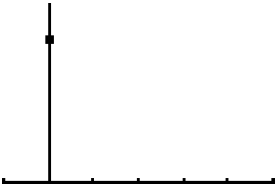
\includegraphics[scale=1.0]{Sections/LinearFunctionsandInterceptsImages/Figure01.png}
	\caption{Graph showing $(0,800)$}
\end{figure}

Notice that this point lies on the output axis (which you should recall is the vertical axis). And that is where the name comes from. If we look at the function’s graph in this window:

\begin{figure}[H]
	\centering
	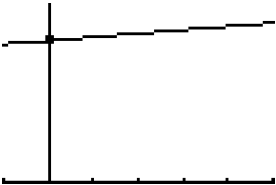
\includegraphics[scale=1.0]{Sections/LinearFunctionsandInterceptsImages/Figure02.png}
	\caption{Graph of $g(x)=20x+800$}
\end{figure}

we can see that this point can be thought of as the place where the graph intersects the vertical axis (i.e. the output axis). And so we call it the vertical intercept.

\exam{\label{LinearFunctionsandInterceptsExample3} A landscaper sells firewood delivered to your home. The price is based on the number of face cords ordered. The formula for the price is given by the function $g(x)=75x+60$.  What is the vertical intercept of this function?
}

\indenttext{The vertical intercept is the \quotes{starting point} for the function, and we know from looking at this example before that the price starts at $\$60$ for delivery and then we add on the cost for the amount of firewood ordered. Using that logic, we know that the vertical intercept is 60.\\
	\newline
	We could also see this from the function itself. We know the vertical intercept is the value you get when your graph hits the vertical (output) axis, which happens when the input value is $x=0$. So, plugging in we would get:
	\begin{equation*}
		g(0)=75(0)+60=60
	\end{equation*}
	which means that the point $(0,60)$ is on the graph, and that the vertical intercept is therefore 60.
}

\bigskip

The term \quotes{vertical intercept} is used a little inconsistently. Sometimes when we say \quotes{vertical intercept} we mean the output value of the function itself, and so in Example \ref{LinearFunctionsandInterceptsExample3} we would say that the vertical intercept is 60. Sometimes, though, when we say \quotes{vertical intercept} we actually mean the point itself where the graph intersects the vertical (output) axis, and so we would say in that case that the vertical intercept is $(0,60)$. Either usage is correct, and it is almost always clear what is meant whichever way you use the term. For Example \ref{LinearFunctionsandInterceptsExample3}, we would have considered either \quotes{$60$} or \quotes{$(0,60)$} a correct answer.

\exam{\label{LinearFunctionsandInterceptsExample4} What is the vertical intercept for the linear function $h(t)=3t-17$?}

\indenttext{Here we don’t know the intended meaning of the function, so we can’t rely on that to tell us the \quotes{starting point}. But we do know that the $y$-intercept happens where the input value is $t=0$. So, substituting in we get:
	\begin{equation*}
		h(0)=3(0)-17=-17
	\end{equation*}
	And so we conclude that the vertical intercept is $-17$. Or, we could equally correctly say that the vertical intercept is $(0, -17)$.
}

\exam{\label{LinearFunctionsandInterceptsExample5} The daily dose of insulin required by a diabetic is a linear function of the grams of carbohydrate consumed. For a particular patient, the daily dose (in units) as required for $x$ grams of carbohydrate is given by the function $f(x)=\frac{1}{6}x+18$.  What is the \quotes{starting amount} of insulin needed before even considering any carbohydrates consumed?
}

\indenttext{This \quotes{starting amount} is the vertical intercept. This would be the amount of insulin needed even if the patient consumed $x=0$ grams. Substituting in we get:
	\begin{equation*}
		f(0)=\frac{1}{6}(0)+18=18
	\end{equation*}
	So the vertical intercept is $18$, which we would interpret here as $18$ units of insulin.
}

\bigskip

It is often very helpful to think of the vertical intercept as the \quotes{starting point}, but sometimes this interpretation is not completely clear, as the following example shows. If a \quotes{starting point} interpretation does not make sense, remember where it comes from. The vertical intercept is the output value of the function when the input is zero. This will be useful in the following example.

\exam{\label{LinearFunctionsandInterceptsExample6} The temperature in degrees Fahrenheit is a linear function of the temperature in degrees Celsius, and is given by the formula $f(C)=\frac{9}{5}C+32$. What is the vertical intercept of this function, and what does it mean in terms of Fahrenheit and Celsius temperatures?
}

\indenttext{
	The vertical intercept is clearly $32$, but it’s not immediately clear what a \quotes{starting point} of $32$ would mean. Remember, though, that this is the output (in degrees Fahrenheit) that you get when the input (in degrees Celsius) is $0$. So, when the input temperature is $0^\circ C$, the output temperature is $32^\circ F$. This doesn’t really lend itself well to a \quotes{starting point} interpretation, but it does make sense - the vertical intercept here is based on the freezing point of water, which happens to be $0^\circ C$.}

\bigskip

Because it is traditional (though as we’ve repeatedly seen certainly not necessary) to call the input variable of a function $x$ and the output variable $y$, the vertical axis can often be called the $y$-axis, and likewise the vertical intercept is often called the $y$-intercept. This is so ingrained that this name is often used even if the output variable has a different name! For example, if we were looking at the linear relationship given by the formula:

\begin{equation*}
	p=3x+12
\end{equation*}

the natural way to look at this would be as defining $p$ as a linear function of $x$. The vertical intercept of this function is 12. Since the output variable is $p$ the vertical (output) axis could also be called the $p$-axis, and it would be reasonable to also call 12 the $p$-intercept. And in fact this is correct usage. Calling it either the \quotes{vertical intercept} or the \quotes{$p$-intercept} would be equally correct, and we will feel free to use either term.\\

It really is not correct to call 12 the \quotes{$y$-intercept} - there is no \quotes{$y$} in this relationship! But it still would not be unusual to hear someone call it the \quotes{$y$-intercept} anyway. We will avoid using the term \quotes{$y$-intercept} unless the output variable actually is named $y$, and you should too! But you also should not be confused, surprised, shocked, or too deeply offended if you run into this mostly harmless misuse of terminology.

%%%%%%%%%%%%%%%%%%%%%%%%%%%%%%%%%%%%%%%%%%%%%%%%%%%%%%%%%%%%%
%
% Subsection: Linear Function and Their Intercepts: Slope-Intercept Form
%
%%%%%%%%%%%%%%%%%%%%%%%%%%%%%%%%%%%%%%%%%%%%%%%%%%%%%%%%%%%%

\subsection{Slope-Intercept Form}

Let’s revisit now the examples we’ve considered. Look at the functions’ formulas and the vertical intercepts:

\begin{center}
	\begin{tabular}{|l|c|c|}
		\hline
		Example & Function Formula & Vertical Intercept\\
		\hline
		Second pool filling example & $g(x)=20x+800$ & 800\\
		\hline
		Delivered Firewood (Example \ref{LinearFunctionsandInterceptsExample3}) & $g(x)=75x+60$ & 60\\
		\hline
		Example \ref{LinearFunctionsandInterceptsExample4} & $h(t)=3t-17$ & -17\\
		\hline
		Insulin Dose (Example \ref{LinearFunctionsandInterceptsExample5} & $f(x)=\frac{1}{6}x+18$ & 18\\
		\hline
	\end{tabular}
\end{center}

The pattern is not hard to see. The vertical intercept seems to always show up in a fairly obvious place in the formula. This is not a coincidence! Think of the logic we used to find the formulas for the pool-filling and firewood-pricing examples. We saw that to figure out the formula, the pattern we needed was:

\begin{equation*}
	f(x)=(slope)x+vertical \text{ } intercept
\end{equation*}

It is not hard to imagine that this would be the case for every linear function, and in fact it is. This leads us to the following conclusion:

\begin{definition}
	\index{Linear Function!Slope-Intercept Form}
	\textbf{\underline{Slope-Intercept Form}}\\
	\bigskip
	A function is linear if and only if its formula can be written in the form
	\begin{equation*}
		f(x)=mx+b
	\end{equation*}
	where $m$ is the slope and $b$ is the vertical intercept.\\
	A formula written in this way is said to be in \textbf{slope-intercept form}.
\end{definition}

(Naturally the names of the function and variable can be different; $g(t)=mt+b$ is also considered to be slope-intercept form.)\\

It is traditional to use the letter $m$ for slope; so much so that usually when you see $m$ used anywhere in math you can usually assume it is meant to be a slope. No one really knows why we use $m$ for slope. At this point it’s just a matter of tradition!\\

Using $b$ for the vertical intercept is also very common. No one really knows why we use the letter $b$ as opposed to some other letter either, but since the vertical intercept is often interpreted as a starting point you can think of it as standing for \quotes{base} or \quotes{beginning}. (That’s not really where it comes from, but it’s a handy thing to remember anyway.)

\exam{\label{LinearFunctionsandInterceptsExample7} the function $h(x)=8x+5$ linear? If so, what is its slope, and what is its vertical intercept?}

\indenttext{The formula for this function is recognizable as being in the $f(x)=mx+b$ form, and so we know it is indeed a linear function. We can see that $m$ is 8 so the slope is 8, and we can see that $b$ is 5 and so the vertical intercept is 5.
}

\bigskip

Combining this slope-intercept form with what we already know about the interpretation of slope and vertical intercept can give us insights into the interpretation of a function from its formula.

\exam{\label{LinearFunctionsandInterceptsExample8} An equipment company rents power equipment by the day. The charge to rent a vibrating tamper for $t$ days is calculated by the function $p(t)=27.5t+15$. Is this function linear? If so, what are the slope and vertical intercept? What do they mean in terms of this equipment rental?
}

\indenttext{The formula for the function fits the slope-intercept ($f(x)=mx+b$) form, with the slope $m$ being $27.5$ and the vertical intercept $b$ being $15$. (The input variable here is $t$ instead of $x$, but the name of the variable doesn’t matter.)\\

	The slope is the rate of change, with units in output units per input unit. So, since the output is cost in dollars and the input is days, the slope is $\$27.50$ per day. The company charges $\$27.50$ per day to rent the tamper.\\

	The vertical intercept is the base, or starting point, and since it is added in as part of the formula to get the output, it must be in the output units. So the vertical intercept is $\$15$. The company starts with a basic charge of $\$15$ to rent the tamper, regardless of how long it is kept out.
}

\bigskip

It is important to note that a function is linear if and only if it's output can be written in slope-intercept ($mx+b$) form. A function that is not written in this form may still be linear, so long as we can put it into this form by simplification.

\exam{\label{LinearFunctionsandInterceptsExample9} Is the function $g(t)=5(t-7)+4t-2(7t-5)$ linear? If so, what is its slope and vertical intercept? If not, how do you know it is not?
}

\indenttext{The function is clearly not currently in slope-intercept ($f(x)=mx+b$) form. But, with some algebraic simplification, we see that it can be rewritten:
	\begin{align*}
		g(t)&=5(t-7)+4t-2(7t-5)\\
		&=5t-35+4t-14t+10\\
		&=-5t-25
	\end{align*}
	Which is very close to slope-intercept form, except that it is a minus sign ($-$) between the terms instead of a addition sign $+$. But we can rewrite this as $g(t)=-5t+(-25)$ which does fit the form with slope $m=-5$ and vertical intercept $b=-25$. So the function is linear.
}

\bigskip

NOTE: Most of the time, we don’t bother rewriting the subtraction as addition of a negative as we did here.  From this point forward, we will just recognize that \quotes{$-5t-25$} is in fact in slope intercept form with a negative vertical intercept without actually bothering to rewrite it as \quotes{$-5t+(-25)$}.

\exam{\label{LinearFunctionsandInterceptsExample10} Is the function $f(x)=2x(4x-5)+3(x-7)$ linear? If so, what is its slope and vertical intercept? If not, how do you know it is not?
}

\indenttext{It certainly is not in slope-intercept form now, but perhaps with some simplification we can get it there:
	\begin{align*}
		f(x) &= 2x(4x-5)+3(x-7) \\
		&=8x^2-10x+3x-21\\
		&=8x^2-7x-21
	\end{align*}

	Here we have reached an impasse. The first term, $8x^2$ contains an exponent, something not allowed in the slope-intercept form. If there were other like terms to combine it with there might be some hope of getting rid of this \quotes{squared} term, but there is none. We cannot simplify this any further, and so we know it cannot be put into slope-intercept form. Therefore this function is not linear.
}

%%%%%%%%%%%%%%%%%%%%%%%%%%%%%%%%%%%%%%%%%%%%%%%%%%%%%%%%%%%%%
%
% Subsection: Linear Function and Their Intercepts: Horizontal Intercept
%
%%%%%%%%%%%%%%%%%%%%%%%%%%%%%%%%%%%%%%%%%%%%%%%%%%%%%%%%%%%%

\subsection{The Horizontal Intercept}

Just as graphs of linear functions intersect the vertical axis, almost every linear function’s graph will intersect the horizontal axis as well. The point where this happens is (not surprisingly) called the \textbf{horizontal intercept} \index{Linear Function!Horizontal Intercept}. Just as the vertical intercept may also be referred to using the name of the output variable, the horizontal intercept may also be referred to using the name of the input variable. And just as the vertical intercept is often incorrectly referred to as the \quotes{$y$-intercept} when the output variable’s name is not $y$, the horizontal intercept is often incorrectly referred to as the \quotes{$x$-intercept} when the input variable’s name is not $x$.\\

The horizontal intercept gets less attention than its vertical cousin. One reason is that, while the very useful slope-intercept form of a linear function’s formula uses the vertical intercept, there is no corresponding useful form using the horizontal intercept. The other reason is that while the vertical intercept is often interpretable as a \quotes{starting point} for the function, the horizontal intercept usually does not lend itself to any natural interpretation.\\

If we do have reason to want to know a linear function’s horizontal intercept, though, it is not all that difficult to find. When we are on the horizontal axis, while we may have moved to the right or left of the origin, we have not moved either up or down. And so the output variable has a value of zero.\\

So, to find the horizontal intercept, we set the output value to zero and determine the input value which makes that happen.\\

The following example will illustrate.

\exam{\label{LinearFunctionsandInterceptsExample11} What is the horizontal intercept for the linear function $f(t)=3t+12$?}

\indenttext{Setting the output value $f$ equal to $0$ we get:

	\begin{equation*}
		f(t)=3t+12\\
		0=3t+12
	\end{equation*}

	an equation we can now solve for $t$:

	\begin{align*}
		0&=3t+12\\
		-3t&=12\\
		t&=-4
	\end{align*}

	And so we conclude that the horizontal intercept is $-4$. Or, equally correctly, we could say that the horizontal intercept is $(-4,0)$. (Note that it is the output value, not the input value, that is $0$.)\\

	It would also be correct to call this the $t$-intercept in this context, since the horizontal (input) axis can be called the $t$-axis since the input variable is $t$. 
}

\bigskip

As far as interpretation of the horizontal intercept is concerned, the important thing is to remember that the horizontal intercept is the input value that makes the output variable equal $0$. Whether or not this is of much interest really depends on whether or not the output variable being equal to $0$ is of much interest. The following example will illustrate.

\exam{\label{LinearFunctionsandInterceptsExample12} Jaye’s electric bill is a function of his electric usage (in kilowatt-hours). The formula used to determine his bill is $f(x)=0.1x+12.5$. Find and interpret
	\begin{enumerate}[label=(\alph*)]
		\item the slope,
		\item the vertical intercept, and
		\item the horizontal intercept of this linear function.
	\end{enumerate} 
}

\indenttext{
	\begin{enumerate}[label=(\alph*)]
		\item The slope can be seen from the fact that the formula is in slope-intercept form. Its units are, as always, output units per input unit. So the slope is $\$0.10$ per kilowatt hour. The slope represents how much he pays for each additional kilowatt hour of electricity used.
		\item The vertical intercept can also be seen from the slope-intercept form. It is $\$12.50$. This would be his bill is his usage were 0 kilowatt hours. So this is a flat rate charged regardless of usage, which he pays just to have electric service to his house.
		\item To find the horizontal intercept, we set the output value to $0$ and solve:

		\begin{align*}
			0&=0.1x+12.5\\
			-0.1x&=12.5\\
			x&=-125
		\end{align*}

		Since the input to this function is electricity usage measured in kilowatt-hours, this horizontal intercept would be interpreted to be $-125$ kilowatt hours.  This would happen if his bill were $\$0$. So, the horizontal intercept is telling us that in order for Jaye to have a $\$0$ electric bill, he would have to use negative 125 kilowatt-hours of electricity.\\

		For most people, this makes no sense at all. You cannot use negative electricity! And probably the horizontal intercept is not of much interest to Jaye.  In this situation we would simply say that there is no practical interpretation of the horizontal intercept in this context.\\

		But, on the other hand, maybe not. If Jaye was mistakenly overbilled last month, it actually might be possible for his electric use to show up as a negative number - to reflect the prior month’s overbilling. Or, if Jaye has solar panels on his roof which generate electricity, it is possible that the panels could generate 125 kilowatt-hours more electricity than he actually uses, resulting in a bill for negative kilowatt-hours.
	\end{enumerate}
}

\bigskip

This example illustrates the horizontal intercept often is not of much interest, but sometimes might be. Jaye probably didn’t get overbilled and probably doesn't have solar panels that produce more electricity than he uses. But, while unlikely, neither of these situations is impossible or absurd. To decide whether or not the horizontal intercept is of any interest, you really need to answer the question \quotes{is it reasonable that the output variable could be zero}. Answering this question will tell you all you need to know about interpreting the horizontal intercept!


%%%%%%%%%%%%%%%%%%%%%%%%%%%%%%%%%%%%%%%%%%%%%%%%%%%%%%%%%%%%
%
% Subsection: Linear Functions and Slope: Exercises
%
%%%%%%%%%%%%%%%%%%%%%%%%%%%%%%%%%%%%%%%%%%%%%%%%%%%%%%%%%%%%

\clearpage
\subsection{Exercises}

\subsubsection*{Vertical Intercept}

\bigskip
\ex{Determine the vertical intercept for each of the following linear functions:
	\begin{enumerate}[label=(\alph*)]
		\item $f(x) = 3x + 5$
		\item $f(t) = -4t + 7$
		\item $g(t) = \frac{5}{2}t - 1$
		\item $f(x) = -7x - \frac{7}{3}$
		\item $h(z) = 4z$
	\end{enumerate}
}
\sol{a. $5$\\b. $7$\\c. $-1$\\d. $-\frac{7}{3}$\\e.$0$}

\bigskip
\ex{Find the vertical intercept for each of the following linear functions:
	\begin{enumerate}[label=(\alph*)]
		\item $h(x) = \frac{7}{3}x + 8$
		\item $f(t) = 3.2t - 1.7$
		\item $g(x) = -\frac{9}{16}x - \frac{3}{7}$
		\item $k(x) = \frac{9}{5}x$
		\item $p(z) = -2z - 7$
	\end{enumerate}
}

\bigskip
\ex{The groundskeeper for a football field is cutting the grass at a steady rate. The total area he has cut (in square yards) $t$ minutes after returning from his morning break is given by the function $a(t) = 25t + 3000$. What is the vertical intercept of this function, and what does it tell you about the groundskeeper and the field?
}
\sol{$3000$; when he began his morning break he had cut $3000$ square feet.}

\bigskip
\ex{A landscaper is producing mulch by loading trimmings into a shredder, which shoots the newly-shredded mulch onto an existing pile. The mulch is being produced at a steady rate. The amount of mulch (in cubic feet) in the pile after $t$ minutes is given by the function $m(t) = \frac{5}{2}t + 378$.  What is the vertical intercept of this function, and what does it tell you about the amount of mulch in the pile?
}

\bigskip
\ex{Driving down the road in my car, I hit my brakes to stop. I slow down at a steady rate and my speed (in miles per hour) as a function of time (in seconds) since I first apply the brakes is given by the formula $s(t) = -3t + 30$. What is the vertical intercept of this function and what does it mean in this scenario?
}
\sol{$30$; when I first hit the brakes I was traveling 30 mph.}

\bigskip
\ex{A motorcycle is accelerating at a constant rate. The speed (in kilometers per hour) as a function of time since the rider hit the gas (in seconds) is given by the formula $v(t) = 0.8t + 42.5$.  What is the vertical intercept of this function and what does it tell you about the motorcycle and its speed?
}

\bigskip
\ex{A wine reviewer is changing the scale she uses for wine ratings. Previously she used a scale where wines were rated on a points scale from 0 to 100 points (though wines were almost never rated below 80 points). In the new scale, wines will be rated from 1 to 5 stars. The new star ratings will correlate to the old points ratings by a linear function. The formula $s = \frac{1}{4} p - 20$ gives the new stars rating as a function of the old points rating. What is the vertical intercept of this function? What does it tell you about her wine ratings?
}
\sol{$-20$; a wine that would have rate 0 points on the old scale would rate $-20$ stars on the new scale.  A rating of $-20$ stars would be weird, but since wines were almost never rated below 80 points, this would actually never happen.  In formal terms, 0 points is in the domain, but not in the relevant domain.}

\bigskip
\ex{Shoe sizes in different parts of the world use different scales. Men’s shoe sizes on the European scale are a linear function of U.S. shoe sizes, and this function is given by the formula $E(s) = \frac{4}{3}s + 30.7$. What is the vertical intercept of this function? What does the vertical intercept tell you about shoe sizes?
}

\bigskip
\ex{The equation $s = 2t + 5$ naturally defines $s$ as a function of $t$. Which of the following statements are true and which are false?
	\begin{enumerate}[label=(\alph*)]
		\item The vertical intercept is 5.
		\item The vertical intercept is $(0,5)$.
		\item The vertical intercept is $(5,0)$.
		\item The $s$-intercept is 5.
		\item The $t$-intercept is 5.
		\item The $y$-intercept is 5.
	\end{enumerate}
}
\sol{a.  true\\b.  true\\c.  false\\d.  true\\e.  false\\f.  false}

\bigskip
\ex{The equation $p = 3x - 7$ defines $p$ as a function of $x$. Which statements are true and
	which are false?
	\begin{enumerate}[label=(\alph*)]
		\item The vertical intercept is 7.
		\item The vertical intercept is -7.
		\item The vertical intercept is $(-7,0)$.
		\item The vertical intercept is $(0,-7)$.
		\item The $y$-intercept is -7.
		\item The $p$-intercept is -7.
		\item The $x$-intercept is -7.
	\end{enumerate}
}

\subsubsection*{Slope-Intercept Form}

\bigskip
\ex{Find the slope and vertical intercept for each of the following linear functions:
	\begin{enumerate}[label=(\alph*)]
		\item $f(x) = 3x - 24$
		\item $f(x) = 6 - 3x$
		\item $f(x) = 100 - 25(2 - x)$
		\item $f(x) = 3x - 2(x + 5) + 7(2x - 1)$
		\item $f(x) = 18(x - 2) + 9(x + 4)$
	\end{enumerate}
}
\sol{a.  slope:  $3$,vertical intercept:  $-24$\\
	b.  slope:  $-3$,vertical intercept:  $6$\\
	c.  slope:  $25$,vertical intercept:  $50$\\
	d.  slope:  $15$,vertical intercept:  $-17$\\
	e.  slope:  $27$,vertical intercept:  $0$}

\bigskip
\ex{Each of the functions given below is linear. Determine each function’s slope and vertical intercept.
	\begin{enumerate}[label=(\alph*)]
		\item $f(x) = 9x + 27$
		\item $g(x) = 3x + 2x - 8$
		\item $f(x) = 1950 + 3(700 - 2x)$
		\item $h(t) = 375 - 32t - 1.5(2t - 60)$
		\item $p(x) = 3(4x - 12) - 4(3x - 9)$
	\end{enumerate}
}

\bigskip
\ex{Some of the functions given below are linear, and some are not. For the linear ones, find
	the slope and vertical intercept. For the non-linear ones, explain how you know that the function is
	not linear.
	\begin{enumerate}[label=(\alph*)]
		\item $f(x) = 100 + 2(x - 5) - 3(x + 10) - 4x$
		\item $f(t) = \frac{2t-7}{3}$
		\item $g(x) = 3x(2x - 1) + 2x(x - 6)$
		\item $h(t) = \frac{5t-3}{4} - \frac{t+1}{2}$
		\item $w(t) = t^2 - t(t + 5) + 1$
		\item $f(x) = x^2 - 2(x + 5) + 1$
	\end{enumerate}
}
\sol{a.  slope:  $-5$,vertical intercept:  $60$\\
	b.  slope:  $\frac{2}{3}$,vertical intercept:  $-\frac{7}{3}$\\
	c.  not a linear function\\
	d.  slope:  $\frac{3}{4}$,vertical intercept:  $-\frac{5}{4}$\\
	e.  slope:  $-5$,vertical intercept:  $1$\\
	f.  not a linear function
}

\bigskip
\ex{Determine whether or not each of the following functions is linear. If the function is linear,
	find the slope and vertical intercept. If the function is not linear, explain how you know that it is
	not.
	\begin{enumerate}[label=(\alph*)]
		\item $g(x) = 2x - 7(2 - x)$
		\item $g(x) = 2x - 7x(2 - x)$
		\item $g(x) = 2 - 7(2 - x)$
		\item $g(x) = 2 - 7x(2 - x)$
		\item $g(x) = \frac{7(2 - x)}{2}$
	\end{enumerate}
}

\bigskip
\ex{A scanning machine is processing a stack of standardized test answer sheets at a constant rate. The number of papers left to process as a function of seconds since the machine began working is given by the function $p(t) = 240 - 3t$. Find and interpret the slope and vertical intercept of this function.
}
\sol{Slope: $-3$; The machine is processing three answer sheets per minute (the number of sheets left to be processed is changing at -3 sheets per minute).\\
	Vertical Intercept: $240$; There were 240 papers to be processed when the machine began working.}

\bigskip
\ex{Paul has a coffee shop gift card he uses every time he stops at his favorite coffee shop. He always orders the same thing and the prices do not change. The amount of money left on a coffee shop gift card is a function of how many times he has visited using this card, and is given by the formula $r(v) = 50 - 3.50v$. Find and interpret the slope and vertical intercept of this function.
}

\bigskip
\ex{Suppose the cost to rent a kayak for $t$ hours is given by $c(t) = 45 + 30(t - 1)$. Is this a linear function? If so, find and interpret its slope and vertical intercept. If not, explain why it is not linear.
}
\sol{Yes, it is a linear function\\
	Slope: $30$; The cost to rent the kayak is increasing at $\$30$ per hour.  Or, in simpler terms, there is a charge of $\$30$ per hour to rent the kayak.\\
	Vertical Intercept: $15$; When you first rent the kayak, there is a $\$15$ charge.  Or, in simpler terms, there is a flat fee charge of $\$15$ in addition to the hourly rate.}

\bigskip
\ex{A hotel reviewer is changing the scale he uses for hotel ratings. Previously he used a scale where hotels were rated on a scale from 0 to 5 stars. On the new scale, hotels will be rated from 0 to 100 points. The new point ratings can be related to the old star ratings using the formula $p = 80 + 5(s - 1)$. Does this formula define a linear function? If so, find and interpret the slope and vertical intercept. If not, explain how you know the function is not linear.
}


\subsubsection*{Horizontal Intercept}

\bigskip
\ex{Find the horizontal intercept for $f(t) = 7t - 84$.}
\sol{$12$ or $(12,0)$}

\bigskip
\ex{Find the horizontal intercept for $f(x) = 2x + 30$.}

\bigskip
\ex{What is the horizontal intercept of $g(x) = 16 + 5x$?}
\sol{$-\frac{16}{5}$ or $(-\frac{16}{5},0)$}

\bigskip
\ex{What is the horizontal intercept of $h(t) = 14 - \frac{5}{2}t$?}

\bigskip
\ex{Driving down the road in my car, I hit my brakes to stop. I slow down at a steady rate and my speed (in miles per hour) as a function of time (in seconds) since I first apply the brakes is given by the formula $s(t) = -3t + 30$. What is the horizontal intercept of this function and what does it mean in this scenario?
}
\sol{$10$; The speed of the car reaches zero (that is; the car comes to a stop) 10 seconds after I hit the brakes.}

\bigskip
\ex{A scanning machine is processing a stack of standardized test answer sheets at a constant rate. The number of papers left to process as a function of seconds since the machine began working is given by the function $p(t) = 240 - 3t$. Find and interpret the horizontal intercept of this function.
}

\bigskip
\ex{A wine reviewer is changing the scale she uses for wine ratings. Previously she used a scale where wines were rated on a points scale from 0 to 100 points (though wines were almost never rated below 80 points). In the new scale, wines will be rated from 1 to 5 stars. The new star ratings will correlate to the old points ratings by a linear function. The formula $s = \frac{1}{4}p - 20$ gives the new stars rating as a function of the old points rating. What is the horizontal intercept of this function? What does it tell you about her wine ratings?
}
\sol{$80$; a wine that would rate 0 stars under the new system would have been rated at 80 points under the old system.}


\subsubsection*{Grab Bag}

\bigskip
\ex{Find the (a) slope, (b) vertical intercept, and (c) horizontal intercept for the linear function $f(x) = 80 - 10x$.}

\bigskip
\ex{Paul has a coffee shop gift card he uses every time he stops at his favorite coffee shop. He always orders the same thing and the prices do not change. The amount of money left on a coffee shop gift card is a function of how many times he has visited using this card, and is given by the formula $r(v) = 50 - 3.50v$. Find and interpret the horizontal intercept of this function.
}
\sol{$14.29$; This would be the number of visits after which his card balance would reach $\$0$.  Since he cannot make a fractional visit, we would interpret this to mean that his card will allow him 14 visits before it is exhausted.}

\bigskip
\ex{Is $f(x) = 6x^2 - 3x(2x - 5)$ linear? If so, determine its slope and vertical intercept. If not, explain how you know it is not.}

\bigskip
\ex{Until it hits the ground below, the speed (in feet per second) of a rock dropped off a bridge is a linear function of the time (in seconds) since it was dropped. The function’s formula is $s(t) = 32t$. Find and interpret the vertical intercept of this function.}
\sol{$0$; The rocks speed when it was dropped was $0$ feet per second.  In other words, the rock was at rest when it began to fall -- it was dropped rather than thrown downward.}

\bigskip
\ex{At the Tastee Lard Bakery, the price of an order for $x$ dozen donuts is $3.25 + 5.75x$.
	\begin{enumerate}[label=(\alph*)]
		\item What is the slope of this function, and what does it tell you about donut prices? 
		\item What is the vertical intercept of this function, and what does it tell you about donut prices? 
		\item What is the horizontal intercept of this function, and what does it tell you about donut prices?
	\end{enumerate} 
}

\bigskip
\ex{Find the (a) slope, (b) vertical intercept, and (c) horizontal intercept for the linear function $p(t) = 35 - 4t$.}
\sol{a.  $-4$\\b.  $35$\\c.  $\frac{35}{4}$}

\bigskip
\ex{If the function $g(x) = 18 - 3(2 - x)$ is linear, find its slope and vertical intercept. If it isn’t, explain how you know that it is not.}

\bigskip
\ex{According to an exercise science textbook, the ideal heart rate for a cardio workout is a linear function of your age. The formula for ideal heart rate as a function of age is $h(a) = 176 - 0.8a$. 
	\begin{enumerate}[label=(\alph*)]
		\item Find and interpret the vertical intercept of this function. 
		\item Find and interpret the horizontal intercept of this function. 
		\item Neither of these intercepts has a realistically useful meaning. Which do you think is the more useless and why? 
	\end{enumerate}
}
\sol{a.  $176$;  The ideal heart rate for a newborn (age 0) would be 176.  This age probably falls outside of the relevant domain of the function since I almost never see newborns using the cardio equipment at the gym, but it can be interpreted as the starting point from which ideal cardio rates decline with age.\\
	b.  $220$; This is the age at which the ideal heart rate reaches zero using this function.  While it is true that most 220 year old people have a heart rate of zero, this probably falls outside of the relevant domain as well.\\
	c.  The horizontal intercept.
}

\bigskip
\ex{Boyan Sea Cruises normally charges $\$2500$ for a 7 day Caribbean cruise, but it offers a discount for customers who refer other people to the cruise line. If you refer $x$ people who also take the cruise, you will pay $2500 - 250x$ dollars for your own cruise.  Find and interpret 
	\begin{enumerate}[label=(\alph*)]
		\item the slope, 
		\item the vertical intercept, and 
		\item the horizontal intercept for this function.
	\end{enumerate}
}

\bigskip
\ex{Rachel does face-painting for kids at fairs and street festivals. The amount of profit she makes as a function of how any face paintings she does in a day is given by the equation $p = 4x - 0.8x - 80$. If this function is linear, find and explain the meaning of (a) its slope, (b) its vertical intercept, and (c) its horizontal intercept. If it is not linear, explain how you know it is not.
}
\sol{Slope: $3.2$; Her profits increase by $\$3.20$ for each face painting that she does.\\
	Vertical Intercept: $-80$; Her profits would be $\$-80$, or in other words she would have a loss of $\$80$ if she did no face painting.  This probably represents how much it costs her for the booth rental, travel, supplies, etc.\\
	c. Horizontal Intercept: $25$; When she does 25 face paintings her profit is $\$0$.  In plainer terms this means that she needs to do 25 face paintings to break even.}

\bigskip
\ex{Sid and Nancy are trying to make sense of their electric bill. The electric company charges them $\$10$ each month for providing electric service, regardless of how much electricity they use, and then $\$0.10$ per kilowatt hour used. \\
	Nancy says that their electric bill is a linear function of their electric usage, because the rate per kilowatt-hour is always the same $\$0.10$.  Since the rate per kilowatt-hour is always the same, the function is linear.\\
	Sid disagrees. Sid calculates that if they use 100 kilowatt-hours they would pay $\$20$, and $\$20$ divided by 100 kilowatt hours is $\$0.20$ per kilowatt-hour. But if they use, say, 400 kilowatt-hours, their bill would be $\$50$, and $\$50$ divided by 400 kilowatt-hours works out to $\$0.125$ per kilowatt-hour. So the rate per kilowatt hour is not always the same, and so it’s not a linear function after all.\\
	Who is right, who is wrong, and where is the mistake in the reasoning of the person who is wrong?
}

\bigskip
\ex{$f(y) = 3y - 12$. What is the $y$-intercept of this function?}
\sol{Since the input variable is $y$, the $y$-intercept in this context is the horizontal intercept of the function which is $4$ or $(4,0)$}

\clearpage
